\documentclass[twoside]{book}

% Packages required by doxygen
\usepackage{fixltx2e}
\usepackage{calc}
\usepackage{doxygen}
\usepackage[export]{adjustbox} % also loads graphicx
\usepackage{graphicx}
\usepackage[utf8]{inputenc}
\usepackage{makeidx}
\usepackage{multicol}
\usepackage{multirow}
\PassOptionsToPackage{warn}{textcomp}
\usepackage{textcomp}
\usepackage[nointegrals]{wasysym}
\usepackage[table]{xcolor}

% Font selection
\usepackage[T1]{fontenc}
\usepackage[scaled=.90]{helvet}
\usepackage{courier}
\usepackage{amssymb}
\usepackage{sectsty}
\renewcommand{\familydefault}{\sfdefault}
\allsectionsfont{%
  \fontseries{bc}\selectfont%
  \color{darkgray}%
}
\renewcommand{\DoxyLabelFont}{%
  \fontseries{bc}\selectfont%
  \color{darkgray}%
}
\newcommand{\+}{\discretionary{\mbox{\scriptsize$\hookleftarrow$}}{}{}}

% Page & text layout
\usepackage{geometry}
\geometry{%
  a4paper,%
  top=2.5cm,%
  bottom=2.5cm,%
  left=2.5cm,%
  right=2.5cm%
}
\tolerance=750
\hfuzz=15pt
\hbadness=750
\setlength{\emergencystretch}{15pt}
\setlength{\parindent}{0cm}
\setlength{\parskip}{3ex plus 2ex minus 2ex}
\makeatletter
\renewcommand{\paragraph}{%
  \@startsection{paragraph}{4}{0ex}{-1.0ex}{1.0ex}{%
    \normalfont\normalsize\bfseries\SS@parafont%
  }%
}
\renewcommand{\subparagraph}{%
  \@startsection{subparagraph}{5}{0ex}{-1.0ex}{1.0ex}{%
    \normalfont\normalsize\bfseries\SS@subparafont%
  }%
}
\makeatother

% Headers & footers
\usepackage{fancyhdr}
\pagestyle{fancyplain}
\fancyhead[LE]{\fancyplain{}{\bfseries\thepage}}
\fancyhead[CE]{\fancyplain{}{}}
\fancyhead[RE]{\fancyplain{}{\bfseries\leftmark}}
\fancyhead[LO]{\fancyplain{}{\bfseries\rightmark}}
\fancyhead[CO]{\fancyplain{}{}}
\fancyhead[RO]{\fancyplain{}{\bfseries\thepage}}
\fancyfoot[LE]{\fancyplain{}{}}
\fancyfoot[CE]{\fancyplain{}{}}
\fancyfoot[RE]{\fancyplain{}{\bfseries\scriptsize Generated by Doxygen }}
\fancyfoot[LO]{\fancyplain{}{\bfseries\scriptsize Generated by Doxygen }}
\fancyfoot[CO]{\fancyplain{}{}}
\fancyfoot[RO]{\fancyplain{}{}}
\renewcommand{\footrulewidth}{0.4pt}
\renewcommand{\chaptermark}[1]{%
  \markboth{#1}{}%
}
\renewcommand{\sectionmark}[1]{%
  \markright{\thesection\ #1}%
}

% Indices & bibliography
\usepackage{natbib}
\usepackage[titles]{tocloft}
\setcounter{tocdepth}{3}
\setcounter{secnumdepth}{5}
\makeindex

% Hyperlinks (required, but should be loaded last)
\usepackage{ifpdf}
\ifpdf
  \usepackage[pdftex,pagebackref=true]{hyperref}
\else
  \usepackage[ps2pdf,pagebackref=true]{hyperref}
\fi
\hypersetup{%
  colorlinks=true,%
  linkcolor=blue,%
  citecolor=blue,%
  unicode%
}

% Custom commands
\newcommand{\clearemptydoublepage}{%
  \newpage{\pagestyle{empty}\cleardoublepage}%
}

\usepackage{caption}
\captionsetup{labelsep=space,justification=centering,font={bf},singlelinecheck=off,skip=4pt,position=top}

%===== C O N T E N T S =====

\begin{document}

% Titlepage & ToC
\hypersetup{pageanchor=false,
             bookmarksnumbered=true,
             pdfencoding=unicode
            }
\pagenumbering{alph}
\begin{titlepage}
\vspace*{7cm}
\begin{center}%
{\Large My Project }\\
\vspace*{1cm}
{\large Generated by Doxygen 1.8.12}\\
\end{center}
\end{titlepage}
\clearemptydoublepage
\pagenumbering{roman}
\tableofcontents
\clearemptydoublepage
\pagenumbering{arabic}
\hypersetup{pageanchor=true}

%--- Begin generated contents ---
\chapter{Hierarchical Index}
\section{Class Hierarchy}
This inheritance list is sorted roughly, but not completely, alphabetically\+:\begin{DoxyCompactList}
\item \contentsline{section}{Chord\+User}{\pageref{class_chord_user}}{}
\item Input\+Stream\begin{DoxyCompactList}
\item \contentsline{section}{File\+Stream}{\pageref{class_file_stream}}{}
\end{DoxyCompactList}
\item Runnable\begin{DoxyCompactList}
\item \contentsline{section}{Shutdown}{\pageref{class_shutdown}}{}
\end{DoxyCompactList}
\item Serializable\begin{DoxyCompactList}
\item \contentsline{section}{File\+Stream}{\pageref{class_file_stream}}{}
\end{DoxyCompactList}
\item Thread\begin{DoxyCompactList}
\item \contentsline{section}{Shutdown}{\pageref{class_shutdown}}{}
\end{DoxyCompactList}
\item Unicast\+Remote\+Object\begin{DoxyCompactList}
\item \contentsline{section}{Chord}{\pageref{class_chord}}{}
\end{DoxyCompactList}
\item Remote\begin{DoxyCompactList}
\item \contentsline{section}{Chord\+Message\+Interface}{\pageref{interface_chord_message_interface}}{}
\begin{DoxyCompactList}
\item \contentsline{section}{Chord}{\pageref{class_chord}}{}
\end{DoxyCompactList}
\item \contentsline{section}{Shutdown\+Interface}{\pageref{interface_shutdown_interface}}{}
\begin{DoxyCompactList}
\item \contentsline{section}{Chord}{\pageref{class_chord}}{}
\end{DoxyCompactList}
\end{DoxyCompactList}
\end{DoxyCompactList}

\chapter{Class Index}
\section{Class List}
Here are the classes, structs, unions and interfaces with brief descriptions\+:\begin{DoxyCompactList}
\item\contentsline{section}{\hyperlink{class_chat}{Chat} \\*It implements a distributed chat. It creates a ring and delivers messages using flooding }{\pageref{class_chat}}{}
\item\contentsline{section}{\hyperlink{class_chat_1_1_client}{Chat.\+Client} \\*It implements the client }{\pageref{class_chat_1_1_client}}{}
\item\contentsline{section}{\hyperlink{enum_chat_1_1enum___m_s_g}{Chat.\+enum\+\_\+\+M\+SG} \\*Enum Class to keep track of message Ids }{\pageref{enum_chat_1_1enum___m_s_g}}{}
\item\contentsline{section}{\hyperlink{class_chat_1_1_main_message}{Chat.\+Main\+Message} \\*This class implements a main message. It keeps all the information the user would like to send to its peers }{\pageref{class_chat_1_1_main_message}}{}
\item\contentsline{section}{\hyperlink{class_chat_1_1_peer}{Chat.\+Peer} \\*This class implements a peer. It keeps the information of our peer simulating a doubly-\/linkedlist }{\pageref{class_chat_1_1_peer}}{}
\item\contentsline{section}{\hyperlink{class_chat_1_1_server}{Chat.\+Server} \\*It implements the server }{\pageref{class_chat_1_1_server}}{}
\end{DoxyCompactList}

\chapter{File Index}
\section{File List}
Here is a list of all files with brief descriptions\+:\begin{DoxyCompactList}
\item\contentsline{section}{C\+E\+C\+S 327/\+C\+E\+C\+S-\/327/\+Assignment\+\_\+2/\hyperlink{_chat_8java}{Chat.\+java} }{\pageref{_chat_8java}}{}
\end{DoxyCompactList}

\chapter{Class Documentation}
\hypertarget{class_chat}{}\section{Chat Class Reference}
\label{class_chat}\index{Chat@{Chat}}


It implements a distributed chat. It creates a ring and delivers messages using flooding.  


Inheritance diagram for Chat\+:\begin{figure}[H]
\begin{center}
\leavevmode
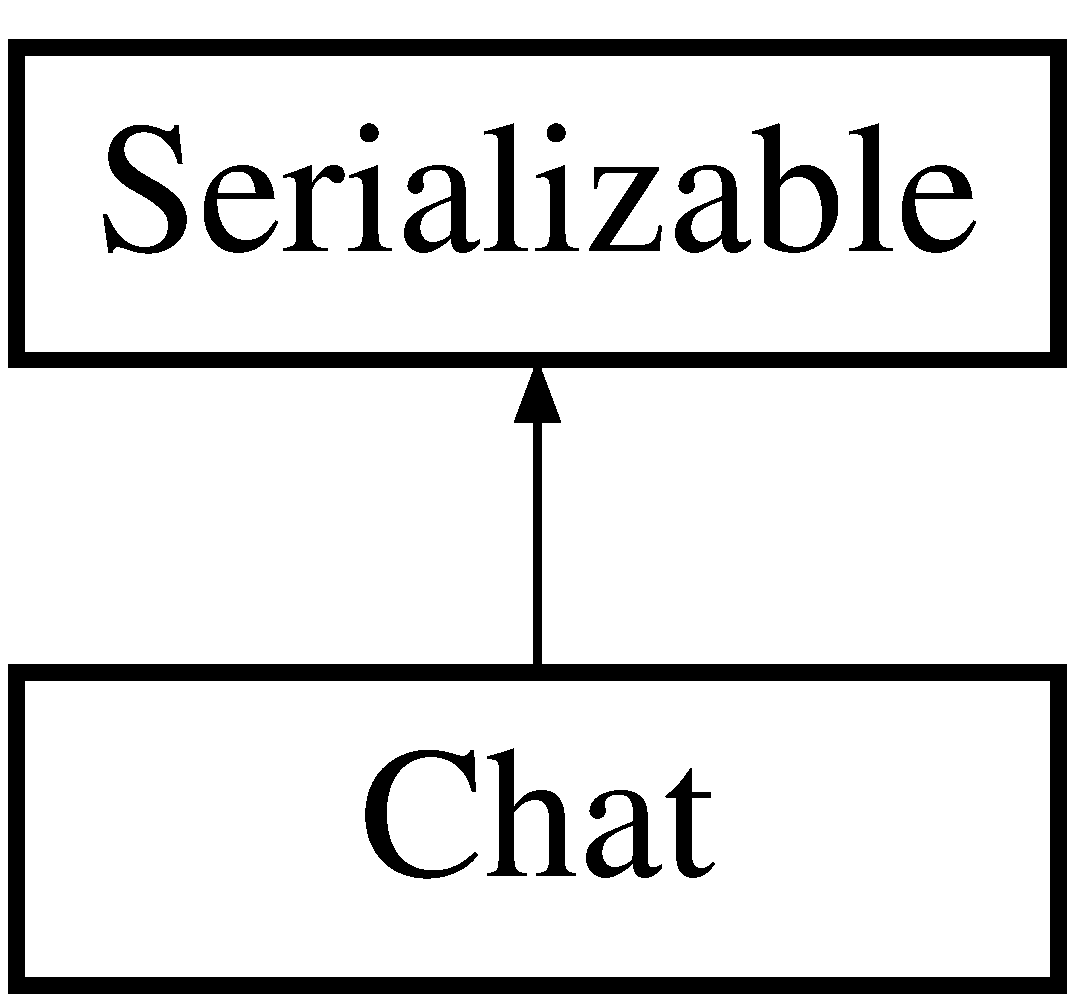
\includegraphics[height=2.000000cm]{class_chat}
\end{center}
\end{figure}
\subsection*{Classes}
\begin{DoxyCompactItemize}
\item 
class \hyperlink{class_chat_1_1_client}{Client}
\begin{DoxyCompactList}\small\item\em It implements the client. \end{DoxyCompactList}\item 
enum \hyperlink{enum_chat_1_1enum___m_s_g}{enum\+\_\+\+M\+SG}
\begin{DoxyCompactList}\small\item\em Enum Class to keep track of message Ids. \end{DoxyCompactList}\item 
class \hyperlink{class_chat_1_1_main_message}{Main\+Message}
\begin{DoxyCompactList}\small\item\em This class implements a main message. It keeps all the information the user would like to send to its peers. \end{DoxyCompactList}\item 
class \hyperlink{class_chat_1_1_peer}{Peer}
\begin{DoxyCompactList}\small\item\em This class implements a peer. It keeps the information of our peer simulating a doubly-\/linkedlist. \end{DoxyCompactList}\item 
class \hyperlink{class_chat_1_1_server}{Server}
\begin{DoxyCompactList}\small\item\em It implements the server. \end{DoxyCompactList}\end{DoxyCompactItemize}
\subsection*{Public Member Functions}
\begin{DoxyCompactItemize}
\item 
\hyperlink{class_chat_a91a76d5af693d46468ee876313ba7afe}{Chat} (String Id, int port)
\end{DoxyCompactItemize}
\subsection*{Static Public Member Functions}
\begin{DoxyCompactItemize}
\item 
static void \hyperlink{class_chat_a04e26027ad460092250efa75ce7a8a19}{main} (String\mbox{[}$\,$\mbox{]} args)
\end{DoxyCompactItemize}


\subsection{Detailed Description}
It implements a distributed chat. It creates a ring and delivers messages using flooding. 

\subsection{Constructor \& Destructor Documentation}
\hypertarget{class_chat_a91a76d5af693d46468ee876313ba7afe}{}\label{class_chat_a91a76d5af693d46468ee876313ba7afe} 
\index{Chat@{Chat}!Chat@{Chat}}
\index{Chat@{Chat}!Chat@{Chat}}
\subsubsection{\texorpdfstring{Chat()}{Chat()}}
{\footnotesize\ttfamily Chat.\+Chat (\begin{DoxyParamCaption}\item[{String}]{Id,  }\item[{int}]{port }\end{DoxyParamCaption})}

Starts the threads with the client and server\+: 
\begin{DoxyParams}{Parameters}
{\em Id} & unique identifier of the process \\
\hline
{\em port} & where the server will listen \\
\hline
\end{DoxyParams}


\subsection{Member Function Documentation}
\hypertarget{class_chat_a04e26027ad460092250efa75ce7a8a19}{}\label{class_chat_a04e26027ad460092250efa75ce7a8a19} 
\index{Chat@{Chat}!main@{main}}
\index{main@{main}!Chat@{Chat}}
\subsubsection{\texorpdfstring{main()}{main()}}
{\footnotesize\ttfamily static void Chat.\+main (\begin{DoxyParamCaption}\item[{String \mbox{[}$\,$\mbox{]}}]{args }\end{DoxyParamCaption})\hspace{0.3cm}{\ttfamily [static]}}



The documentation for this class was generated from the following file\+:\begin{DoxyCompactItemize}
\item 
C\+E\+C\+S 327/\+C\+E\+C\+S-\/327/\+Assignment\+\_\+2/\hyperlink{_chat_8java}{Chat.\+java}\end{DoxyCompactItemize}

\hypertarget{class_chat_1_1_client}{}\section{Chat.\+Client Class Reference}
\label{class_chat_1_1_client}\index{Chat.\+Client@{Chat.\+Client}}


It implements the client.  


Inheritance diagram for Chat.\+Client\+:\begin{figure}[H]
\begin{center}
\leavevmode
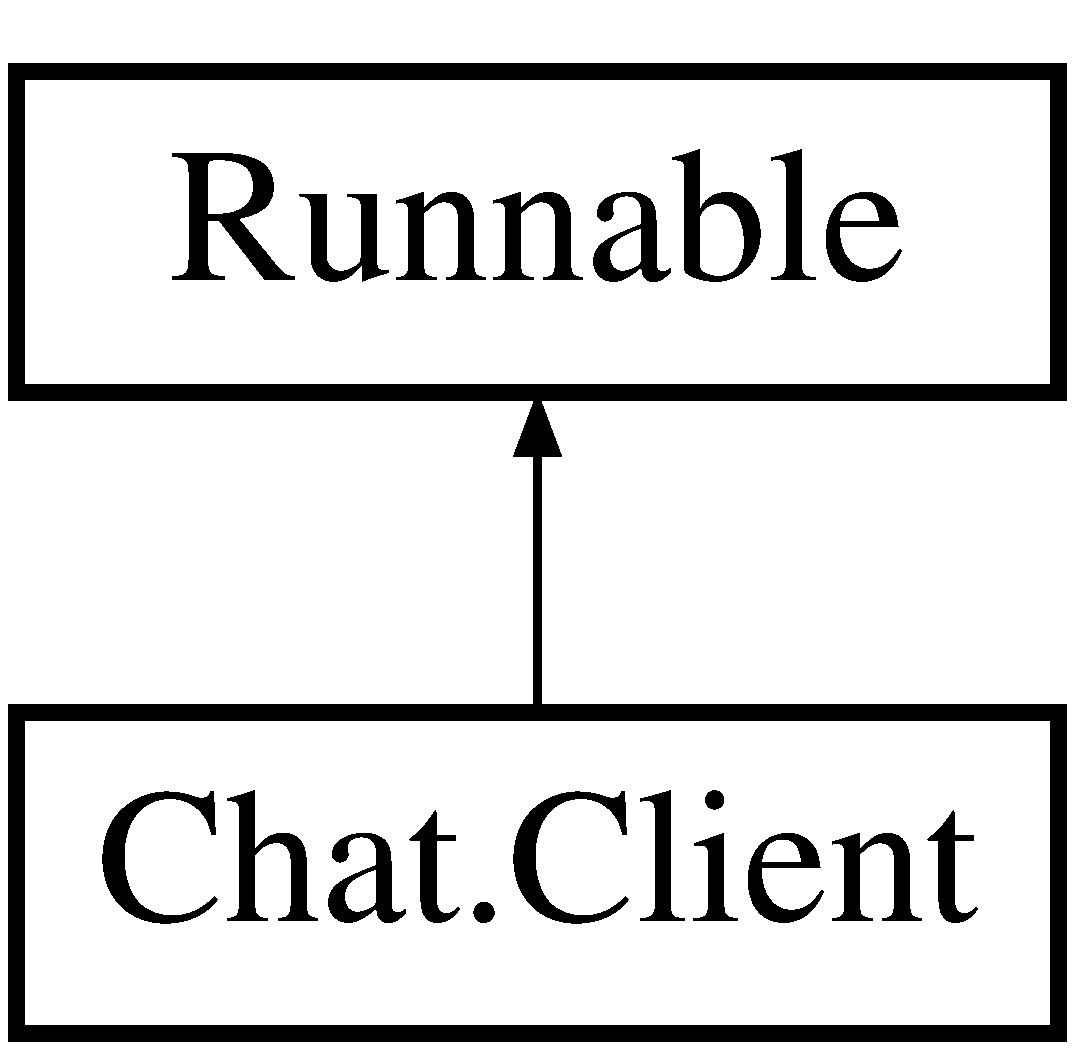
\includegraphics[height=2.000000cm]{class_chat_1_1_client}
\end{center}
\end{figure}
\subsection*{Public Member Functions}
\begin{DoxyCompactItemize}
\item 
\hyperlink{class_chat_1_1_client_a4d66bd0f3bc141314127bc43806cbe6e}{Client} (String id, int p)
\item 
void \hyperlink{class_chat_1_1_client_af929f8bd324136e11afe64c92fa1cac3}{run} ()
\begin{DoxyCompactList}\small\item\em It allows the user to interact with the system. \end{DoxyCompactList}\end{DoxyCompactItemize}


\subsection{Detailed Description}
It implements the client. 

class \hyperlink{class_chat_1_1_client}{Client} class \char`\"{}chat.\+java\char`\"{} 

\subsection{Constructor \& Destructor Documentation}
\hypertarget{class_chat_1_1_client_a4d66bd0f3bc141314127bc43806cbe6e}{}\label{class_chat_1_1_client_a4d66bd0f3bc141314127bc43806cbe6e} 
\index{Chat\+::\+Client@{Chat\+::\+Client}!Client@{Client}}
\index{Client@{Client}!Chat\+::\+Client@{Chat\+::\+Client}}
\subsubsection{\texorpdfstring{Client()}{Client()}}
{\footnotesize\ttfamily Chat.\+Client.\+Client (\begin{DoxyParamCaption}\item[{String}]{id,  }\item[{int}]{p }\end{DoxyParamCaption})}



\subsection{Member Function Documentation}
\hypertarget{class_chat_1_1_client_af929f8bd324136e11afe64c92fa1cac3}{}\label{class_chat_1_1_client_af929f8bd324136e11afe64c92fa1cac3} 
\index{Chat\+::\+Client@{Chat\+::\+Client}!run@{run}}
\index{run@{run}!Chat\+::\+Client@{Chat\+::\+Client}}
\subsubsection{\texorpdfstring{run()}{run()}}
{\footnotesize\ttfamily void Chat.\+Client.\+run (\begin{DoxyParamCaption}{ }\end{DoxyParamCaption})}



It allows the user to interact with the system. 



The documentation for this class was generated from the following file\+:\begin{DoxyCompactItemize}
\item 
C\+E\+C\+S 327/\+C\+E\+C\+S-\/327/\+Assignment\+\_\+2/\hyperlink{_chat_8java}{Chat.\+java}\end{DoxyCompactItemize}

\hypertarget{enum_chat_1_1enum___m_s_g}{}\section{Chat.\+enum\+\_\+\+M\+SG Enum Reference}
\label{enum_chat_1_1enum___m_s_g}\index{Chat.\+enum\+\_\+\+M\+SG@{Chat.\+enum\+\_\+\+M\+SG}}


Enum Class to keep track of message Ids.  


\subsection*{Public Attributes}
\begin{DoxyCompactItemize}
\item 
\hyperlink{enum_chat_1_1enum___m_s_g_a13207b3d66634728aa90ddeaba3c07b2}{J\+O\+IN}
\item 
\hyperlink{enum_chat_1_1enum___m_s_g_a10c727775b1daf320c5e7c55cfce0c75}{A\+C\+C\+E\+PT}
\item 
\hyperlink{enum_chat_1_1enum___m_s_g_a03d71ee0b5ffa0a67aad84965832d42d}{A\+C\+C\+E\+P\+T\+ED}
\item 
\hyperlink{enum_chat_1_1enum___m_s_g_ad6d5aef8d11c44afb9c929bcad90dcaa}{L\+E\+A\+VE}
\item 
\hyperlink{enum_chat_1_1enum___m_s_g_afe9c3f90691c6e27ce6f063b24c2ba3c}{P\+UT}
\end{DoxyCompactItemize}


\subsection{Detailed Description}
Enum Class to keep track of message Ids. 

\subsection{Member Data Documentation}
\hypertarget{enum_chat_1_1enum___m_s_g_a10c727775b1daf320c5e7c55cfce0c75}{}\label{enum_chat_1_1enum___m_s_g_a10c727775b1daf320c5e7c55cfce0c75} 
\index{Chat\+::enum\+\_\+\+M\+SG@{Chat\+::enum\+\_\+\+M\+SG}!A\+C\+C\+E\+PT@{A\+C\+C\+E\+PT}}
\index{A\+C\+C\+E\+PT@{A\+C\+C\+E\+PT}!Chat\+::enum\+\_\+\+M\+SG@{Chat\+::enum\+\_\+\+M\+SG}}
\subsubsection{\texorpdfstring{A\+C\+C\+E\+PT}{ACCEPT}}
{\footnotesize\ttfamily Chat.\+enum\+\_\+\+M\+S\+G.\+A\+C\+C\+E\+PT}

Accept member \hypertarget{enum_chat_1_1enum___m_s_g_a03d71ee0b5ffa0a67aad84965832d42d}{}\label{enum_chat_1_1enum___m_s_g_a03d71ee0b5ffa0a67aad84965832d42d} 
\index{Chat\+::enum\+\_\+\+M\+SG@{Chat\+::enum\+\_\+\+M\+SG}!A\+C\+C\+E\+P\+T\+ED@{A\+C\+C\+E\+P\+T\+ED}}
\index{A\+C\+C\+E\+P\+T\+ED@{A\+C\+C\+E\+P\+T\+ED}!Chat\+::enum\+\_\+\+M\+SG@{Chat\+::enum\+\_\+\+M\+SG}}
\subsubsection{\texorpdfstring{A\+C\+C\+E\+P\+T\+ED}{ACCEPTED}}
{\footnotesize\ttfamily Chat.\+enum\+\_\+\+M\+S\+G.\+A\+C\+C\+E\+P\+T\+ED}

Send Acceptance to Circle \hypertarget{enum_chat_1_1enum___m_s_g_a13207b3d66634728aa90ddeaba3c07b2}{}\label{enum_chat_1_1enum___m_s_g_a13207b3d66634728aa90ddeaba3c07b2} 
\index{Chat\+::enum\+\_\+\+M\+SG@{Chat\+::enum\+\_\+\+M\+SG}!J\+O\+IN@{J\+O\+IN}}
\index{J\+O\+IN@{J\+O\+IN}!Chat\+::enum\+\_\+\+M\+SG@{Chat\+::enum\+\_\+\+M\+SG}}
\subsubsection{\texorpdfstring{J\+O\+IN}{JOIN}}
{\footnotesize\ttfamily Chat.\+enum\+\_\+\+M\+S\+G.\+J\+O\+IN}

Join Circle \hypertarget{enum_chat_1_1enum___m_s_g_ad6d5aef8d11c44afb9c929bcad90dcaa}{}\label{enum_chat_1_1enum___m_s_g_ad6d5aef8d11c44afb9c929bcad90dcaa} 
\index{Chat\+::enum\+\_\+\+M\+SG@{Chat\+::enum\+\_\+\+M\+SG}!L\+E\+A\+VE@{L\+E\+A\+VE}}
\index{L\+E\+A\+VE@{L\+E\+A\+VE}!Chat\+::enum\+\_\+\+M\+SG@{Chat\+::enum\+\_\+\+M\+SG}}
\subsubsection{\texorpdfstring{L\+E\+A\+VE}{LEAVE}}
{\footnotesize\ttfamily Chat.\+enum\+\_\+\+M\+S\+G.\+L\+E\+A\+VE}

Leave Circle \hypertarget{enum_chat_1_1enum___m_s_g_afe9c3f90691c6e27ce6f063b24c2ba3c}{}\label{enum_chat_1_1enum___m_s_g_afe9c3f90691c6e27ce6f063b24c2ba3c} 
\index{Chat\+::enum\+\_\+\+M\+SG@{Chat\+::enum\+\_\+\+M\+SG}!P\+UT@{P\+UT}}
\index{P\+UT@{P\+UT}!Chat\+::enum\+\_\+\+M\+SG@{Chat\+::enum\+\_\+\+M\+SG}}
\subsubsection{\texorpdfstring{P\+UT}{PUT}}
{\footnotesize\ttfamily Chat.\+enum\+\_\+\+M\+S\+G.\+P\+UT}

Send a message 

The documentation for this enum was generated from the following file\+:\begin{DoxyCompactItemize}
\item 
C\+E\+C\+S 327/\+C\+E\+C\+S-\/327/\+Assignment\+\_\+2/\hyperlink{_chat_8java}{Chat.\+java}\end{DoxyCompactItemize}

\hypertarget{class_chat_1_1_main_message}{}\section{Chat.\+Main\+Message Class Reference}
\label{class_chat_1_1_main_message}\index{Chat.\+Main\+Message@{Chat.\+Main\+Message}}


This class implements a main message. It keeps all the information the user would like to send to its peers.  


Inheritance diagram for Chat.\+Main\+Message\+:\begin{figure}[H]
\begin{center}
\leavevmode
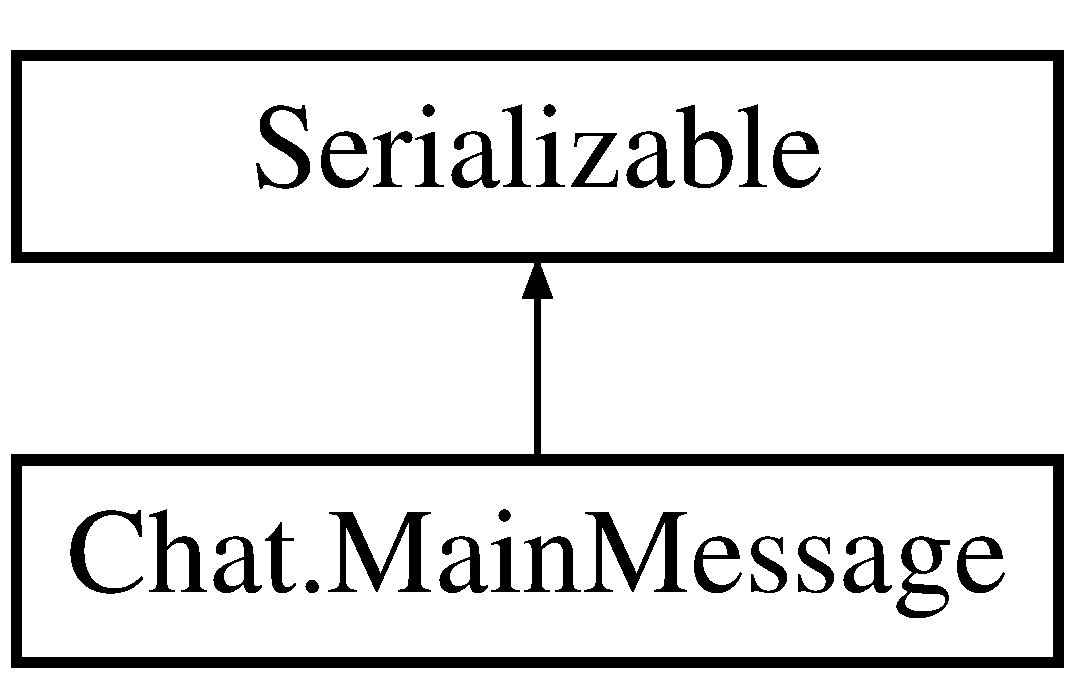
\includegraphics[height=2.000000cm]{class_chat_1_1_main_message}
\end{center}
\end{figure}
\subsection*{Public Member Functions}
\begin{DoxyCompactItemize}
\item 
\hyperlink{class_chat_1_1_main_message_a93ad4ec0e9bf91aa5aa264fd98b44db2}{Main\+Message} (\hyperlink{enum_chat_1_1enum___m_s_g}{enum\+\_\+\+M\+SG} m)
\end{DoxyCompactItemize}


\subsection{Detailed Description}
This class implements a main message. It keeps all the information the user would like to send to its peers. 

\subsection{Constructor \& Destructor Documentation}
\hypertarget{class_chat_1_1_main_message_a93ad4ec0e9bf91aa5aa264fd98b44db2}{}\label{class_chat_1_1_main_message_a93ad4ec0e9bf91aa5aa264fd98b44db2} 
\index{Chat\+::\+Main\+Message@{Chat\+::\+Main\+Message}!Main\+Message@{Main\+Message}}
\index{Main\+Message@{Main\+Message}!Chat\+::\+Main\+Message@{Chat\+::\+Main\+Message}}
\subsubsection{\texorpdfstring{Main\+Message()}{MainMessage()}}
{\footnotesize\ttfamily Chat.\+Main\+Message.\+Main\+Message (\begin{DoxyParamCaption}\item[{\hyperlink{enum_chat_1_1enum___m_s_g}{enum\+\_\+\+M\+SG}}]{m }\end{DoxyParamCaption})}



The documentation for this class was generated from the following file\+:\begin{DoxyCompactItemize}
\item 
C\+E\+C\+S 327/\+C\+E\+C\+S-\/327/\+Assignment\+\_\+2/\hyperlink{_chat_8java}{Chat.\+java}\end{DoxyCompactItemize}

\hypertarget{class_chat_1_1_peer}{}\section{Chat.\+Peer Class Reference}
\label{class_chat_1_1_peer}\index{Chat.\+Peer@{Chat.\+Peer}}


This class implements a peer. It keeps the information of our peer simulating a doubly-\/linkedlist.  


\subsection*{Public Member Functions}
\begin{DoxyCompactItemize}
\item 
\hyperlink{class_chat_1_1_peer_a1ec840ef8993a9ac190db6d6f92b6c01}{Peer} (String id, String ip, int port)
\item 
\hyperlink{class_chat_1_1_peer_a9375050c0c6930ac28dc49cd9ded1029}{Peer} (String id, int port)
\end{DoxyCompactItemize}


\subsection{Detailed Description}
This class implements a peer. It keeps the information of our peer simulating a doubly-\/linkedlist. 

\subsection{Constructor \& Destructor Documentation}
\hypertarget{class_chat_1_1_peer_a1ec840ef8993a9ac190db6d6f92b6c01}{}\label{class_chat_1_1_peer_a1ec840ef8993a9ac190db6d6f92b6c01} 
\index{Chat\+::\+Peer@{Chat\+::\+Peer}!Peer@{Peer}}
\index{Peer@{Peer}!Chat\+::\+Peer@{Chat\+::\+Peer}}
\subsubsection{\texorpdfstring{Peer()}{Peer()}\hspace{0.1cm}{\footnotesize\ttfamily [1/2]}}
{\footnotesize\ttfamily Chat.\+Peer.\+Peer (\begin{DoxyParamCaption}\item[{String}]{id,  }\item[{String}]{ip,  }\item[{int}]{port }\end{DoxyParamCaption})}

\hypertarget{class_chat_1_1_peer_a9375050c0c6930ac28dc49cd9ded1029}{}\label{class_chat_1_1_peer_a9375050c0c6930ac28dc49cd9ded1029} 
\index{Chat\+::\+Peer@{Chat\+::\+Peer}!Peer@{Peer}}
\index{Peer@{Peer}!Chat\+::\+Peer@{Chat\+::\+Peer}}
\subsubsection{\texorpdfstring{Peer()}{Peer()}\hspace{0.1cm}{\footnotesize\ttfamily [2/2]}}
{\footnotesize\ttfamily Chat.\+Peer.\+Peer (\begin{DoxyParamCaption}\item[{String}]{id,  }\item[{int}]{port }\end{DoxyParamCaption})}



The documentation for this class was generated from the following file\+:\begin{DoxyCompactItemize}
\item 
C\+E\+C\+S 327/\+C\+E\+C\+S-\/327/\+Assignment\+\_\+2/\hyperlink{_chat_8java}{Chat.\+java}\end{DoxyCompactItemize}

\hypertarget{class_chat_1_1_server}{}\section{Chat.\+Server Class Reference}
\label{class_chat_1_1_server}\index{Chat.\+Server@{Chat.\+Server}}


It implements the server.  


Inheritance diagram for Chat.\+Server\+:\begin{figure}[H]
\begin{center}
\leavevmode
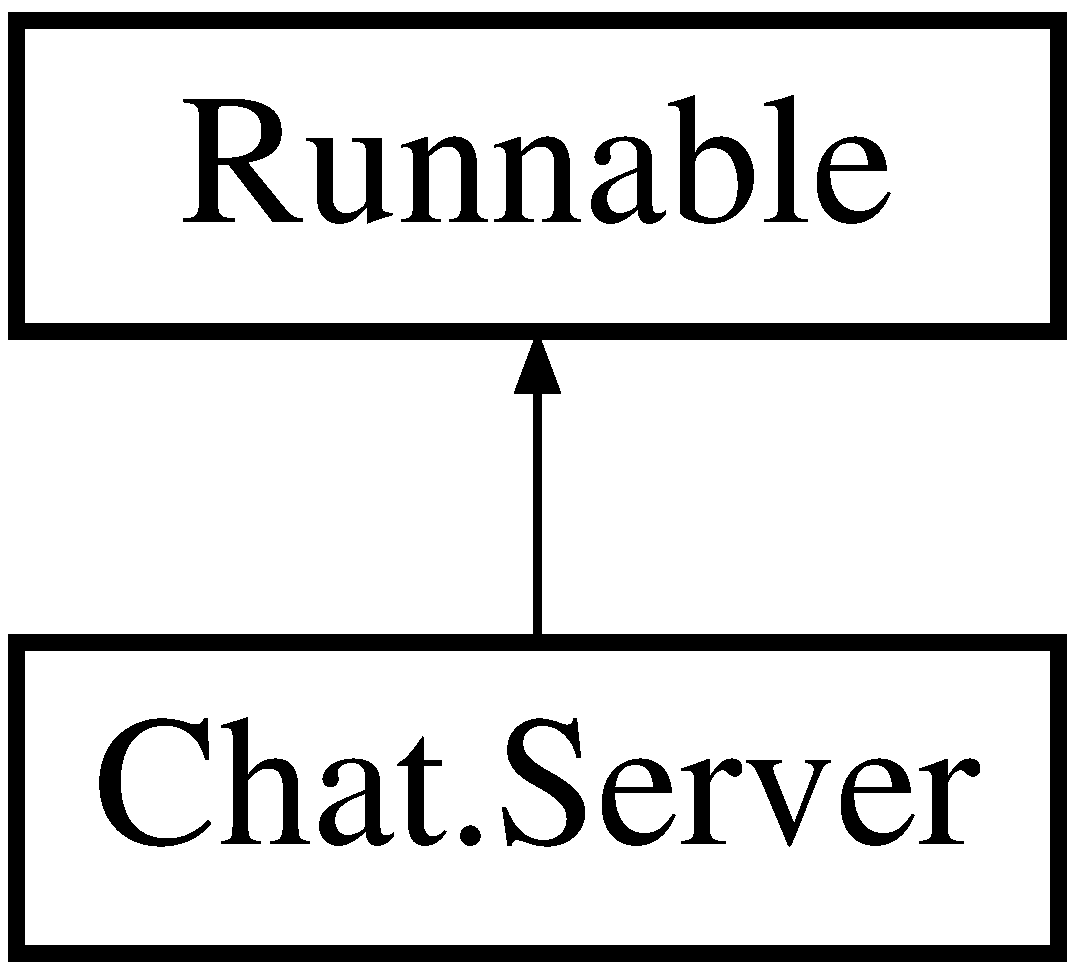
\includegraphics[height=2.000000cm]{class_chat_1_1_server}
\end{center}
\end{figure}
\subsection*{Public Member Functions}
\begin{DoxyCompactItemize}
\item 
\hyperlink{class_chat_1_1_server_a40ee17c05416aed06445215afb74effe}{Server} (String id, int port)
\item 
void \hyperlink{class_chat_1_1_server_a90f3bd24ca99aa3ebf510d1f41b245c3}{run} ()
\begin{DoxyCompactList}\small\item\em It allows the system to interact with the participants. \end{DoxyCompactList}\end{DoxyCompactItemize}


\subsection{Detailed Description}
It implements the server. 

\subsection{Constructor \& Destructor Documentation}
\hypertarget{class_chat_1_1_server_a40ee17c05416aed06445215afb74effe}{}\label{class_chat_1_1_server_a40ee17c05416aed06445215afb74effe} 
\index{Chat\+::\+Server@{Chat\+::\+Server}!Server@{Server}}
\index{Server@{Server}!Chat\+::\+Server@{Chat\+::\+Server}}
\subsubsection{\texorpdfstring{Server()}{Server()}}
{\footnotesize\ttfamily Chat.\+Server.\+Server (\begin{DoxyParamCaption}\item[{String}]{id,  }\item[{int}]{port }\end{DoxyParamCaption})}



\subsection{Member Function Documentation}
\hypertarget{class_chat_1_1_server_a90f3bd24ca99aa3ebf510d1f41b245c3}{}\label{class_chat_1_1_server_a90f3bd24ca99aa3ebf510d1f41b245c3} 
\index{Chat\+::\+Server@{Chat\+::\+Server}!run@{run}}
\index{run@{run}!Chat\+::\+Server@{Chat\+::\+Server}}
\subsubsection{\texorpdfstring{run()}{run()}}
{\footnotesize\ttfamily void Chat.\+Server.\+run (\begin{DoxyParamCaption}{ }\end{DoxyParamCaption})}



It allows the system to interact with the participants. 

get ip from client socket and set to message 

The documentation for this class was generated from the following file\+:\begin{DoxyCompactItemize}
\item 
C\+E\+C\+S 327/\+C\+E\+C\+S-\/327/\+Assignment\+\_\+2/\hyperlink{_chat_8java}{Chat.\+java}\end{DoxyCompactItemize}

\chapter{File Documentation}
\hypertarget{_chat_8java}{}\section{C\+E\+CS 327/\+C\+E\+C\+S-\/327/\+Assignment\+\_\+2/\+Chat.java File Reference}
\label{_chat_8java}\index{C\+E\+C\+S 327/\+C\+E\+C\+S-\/327/\+Assignment\+\_\+2/\+Chat.\+java@{C\+E\+C\+S 327/\+C\+E\+C\+S-\/327/\+Assignment\+\_\+2/\+Chat.\+java}}
\subsection*{Classes}
\begin{DoxyCompactItemize}
\item 
class \hyperlink{class_chat}{Chat}
\begin{DoxyCompactList}\small\item\em It implements a distributed chat. It creates a ring and delivers messages using flooding. \end{DoxyCompactList}\item 
enum \hyperlink{enum_chat_1_1enum___m_s_g}{Chat.\+enum\+\_\+\+M\+SG}
\begin{DoxyCompactList}\small\item\em Enum Class to keep track of message Ids. \end{DoxyCompactList}\item 
class \hyperlink{class_chat_1_1_peer}{Chat.\+Peer}
\begin{DoxyCompactList}\small\item\em This class implements a peer. It keeps the information of our peer simulating a doubly-\/linkedlist. \end{DoxyCompactList}\item 
class \hyperlink{class_chat_1_1_main_message}{Chat.\+Main\+Message}
\begin{DoxyCompactList}\small\item\em This class implements a main message. It keeps all the information the user would like to send to its peers. \end{DoxyCompactList}\item 
class \hyperlink{class_chat_1_1_server}{Chat.\+Server}
\begin{DoxyCompactList}\small\item\em It implements the server. \end{DoxyCompactList}\item 
class \hyperlink{class_chat_1_1_client}{Chat.\+Client}
\begin{DoxyCompactList}\small\item\em It implements the client. \end{DoxyCompactList}\end{DoxyCompactItemize}

%--- End generated contents ---

% Index
\backmatter
\newpage
\phantomsection
\clearemptydoublepage
\addcontentsline{toc}{chapter}{Index}
\printindex

\end{document}
